\documentclass{article}\usepackage[]{graphicx}\usepackage[]{color}
%% maxwidth is the original width if it is less than linewidth
%% otherwise use linewidth (to make sure the graphics do not exceed the margin)
\makeatletter
\def\maxwidth{ %
  \ifdim\Gin@nat@width>\linewidth
    \linewidth
  \else
    \Gin@nat@width
  \fi
}
\makeatother

\definecolor{fgcolor}{rgb}{0.345, 0.345, 0.345}
\newcommand{\hlnum}[1]{\textcolor[rgb]{0.686,0.059,0.569}{#1}}%
\newcommand{\hlstr}[1]{\textcolor[rgb]{0.192,0.494,0.8}{#1}}%
\newcommand{\hlcom}[1]{\textcolor[rgb]{0.678,0.584,0.686}{\textit{#1}}}%
\newcommand{\hlopt}[1]{\textcolor[rgb]{0,0,0}{#1}}%
\newcommand{\hlstd}[1]{\textcolor[rgb]{0.345,0.345,0.345}{#1}}%
\newcommand{\hlkwa}[1]{\textcolor[rgb]{0.161,0.373,0.58}{\textbf{#1}}}%
\newcommand{\hlkwb}[1]{\textcolor[rgb]{0.69,0.353,0.396}{#1}}%
\newcommand{\hlkwc}[1]{\textcolor[rgb]{0.333,0.667,0.333}{#1}}%
\newcommand{\hlkwd}[1]{\textcolor[rgb]{0.737,0.353,0.396}{\textbf{#1}}}%

\usepackage{framed}
\makeatletter
\newenvironment{kframe}{%
 \def\at@end@of@kframe{}%
 \ifinner\ifhmode%
  \def\at@end@of@kframe{\end{minipage}}%
  \begin{minipage}{\columnwidth}%
 \fi\fi%
 \def\FrameCommand##1{\hskip\@totalleftmargin \hskip-\fboxsep
 \colorbox{shadecolor}{##1}\hskip-\fboxsep
     % There is no \\@totalrightmargin, so:
     \hskip-\linewidth \hskip-\@totalleftmargin \hskip\columnwidth}%
 \MakeFramed {\advance\hsize-\width
   \@totalleftmargin\z@ \linewidth\hsize
   \@setminipage}}%
 {\par\unskip\endMakeFramed%
 \at@end@of@kframe}
\makeatother

\definecolor{shadecolor}{rgb}{.97, .97, .97}
\definecolor{messagecolor}{rgb}{0, 0, 0}
\definecolor{warningcolor}{rgb}{1, 0, 1}
\definecolor{errorcolor}{rgb}{1, 0, 0}
\newenvironment{knitrout}{}{} % an empty environment to be redefined in TeX

\usepackage{alltt}
\usepackage{amsmath,amsfonts,bm,fullpage,subcaption,graphicx,caption}
\usepackage{natbib,tikz}
\bibliographystyle{abbrvnat}
\newcommand{\ProjMean}{{\widehat{\bm S}_{2}}}
\newcommand{\GeomMean}{{\widehat{\bm S}_{2,R}}}
\newcommand{\R}{{\mathbb{R}}}
\IfFileExists{upquote.sty}{\usepackage{upquote}}{}
\begin{document}




This simulation design is similar in spirit to Ko and Chang (1993)-\textit{Robust M-Estimators on Spheres}.  Simulation parameters:
\begin{enumerate}
\item Data generted from a $\epsilon$-contaminated distribution:
\[
F=(1-\epsilon)\text{Cayley}(\bm S,40)+\epsilon\text{Cayley}(\bm S^*,20)
\]
\item $\epsilon=0.05, 0.1, 0.15, 0.20$
\item $\bm S=\bm I_{3\times 3}$ and $\bm S^*$ is orthogonal to $\bm S$ (rotated through $\pi/2$ radians) or on the opposite pole (rotated through $\pi$ radians).
\item Sample size: $n=20,50,100$
\end{enumerate}

The median and mean are the usual minimizes of the first- and second-order distances, respectively.  The trimmed mean is found by the following process:
\begin{enumerate}
\item Find the usual mean 
\item Compute the distance between each observation and the estimated mean
\item Remove 10\% observations that are the furthers from the estimated mean
\end{enumerate}

The winsorized mean is computed in the same way, except instead of removing the upper 10\%, they are projected back closer to the estimated mean.

\begin{figure}
\begin{center}
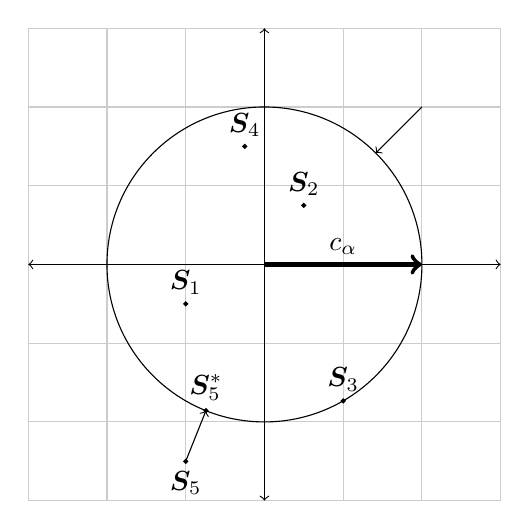
\begin{tikzpicture}
    \draw [black!20] (-3,-3) grid (3,3);
    \draw (0,0) circle [radius=2];
    \draw [->,ultra thick] (0,0) -- (2,0);
    \draw [<->] (-3,0) -- (3,0);
    \draw [<->] (0,-3) -- (0,3);
    %\node [above] at (3,0) {$x$}
    \node [above] at (1,0) {$c_\alpha$};
    \node [above] at (-1,-.5) {$\bm{S}_1$};
    \draw [fill] (-1,-.5) circle [radius=0.025];
    \node [above] at (.5,.75) {$\bm{S}_2$};
    \draw [fill] (.5,.75) circle [radius=0.025];
    \node [above] at (1,-1.732051) {$\bm{S}_3$};
    \draw [fill] (1,-1.732051) circle [radius=0.025];
    \node [above] at (-.25,1.5) {$\bm{S}_4$};
    \draw [fill] (-.25,1.5) circle [radius=0.025];
    %\node [above] at (2,2) {$\bm{S}_5$};
    %\draw [fill] (2,2) circle [radius=0.025];
    %\node [left] at (1.414214, 1.414214) {$\bm{S}_5^*$};
    %\draw [fill] (1.414214, 1.414214) circle [radius=0.025];
    \draw [->] (2,2) -- (1.414214, 1.414214);
    \node [below] at (-1,-2.5) {$\bm{S}_5$};
    \draw [fill] (-1,-2.5) circle [radius=0.025];
    \node [above] at (-0.7427814,  -1.8569534) {$\bm{S}_5^*$};
    \draw [fill] (-0.7427814, -1.8569534) circle [radius=0.025];
    \draw [->] (-1,-2.5) -- (-0.7427814,  -1.8569534);
\end{tikzpicture}
\end{center}
\caption{Winsorized mean estimator where $c_\alpha$ is the $(1-\alpha)100\%$ radius.}
\label{fig:Huber}
\end{figure}

\begin{knitrout}
\definecolor{shadecolor}{rgb}{0.969, 0.969, 0.969}\color{fgcolor}\begin{figure}[]


{\centering \includegraphics[width=1\textwidth]{Figures/method1} 
\includegraphics[width=1\textwidth]{Figures/method2} 

}

\caption[Comparison of contamination central orientations within the estimator methods (extrinsic/intrinsic)]{Comparison of contamination central orientations within the estimator methods (extrinsic/intrinsic).\label{fig:method}}
\end{figure}


\end{knitrout}


\begin{knitrout}
\definecolor{shadecolor}{rgb}{0.969, 0.969, 0.969}\color{fgcolor}\begin{figure}[]


{\centering \includegraphics[width=1\textwidth]{Figures/contam1} 
\includegraphics[width=1\textwidth]{Figures/contam2} 

}

\caption[Comparison of estimator methods (extrinsic/intrinsic) within contamination central orientations]{Comparison of estimator methods (extrinsic/intrinsic) within contamination central orientations.\label{fig:contam}}
\end{figure}


\end{knitrout}



\end{document}
